\section{Box and Whisker plots (aka Box Plot)}\label{Box and Whisker plots (aka Box Plot)}
A box plot or boxplot is a method for demonstrating graphically the locality, spread and skewness groups of numerical data through their quartiles. In addition to the box on a box plot, there can be lines (which are called whiskers) extending from the box indicating variability outside the upper and lower quartiles, thus, the plot is also called the box-and-whisker plot and the box-and-whisker diagram. Outliers that differ significantly from the rest of the dataset may be plotted as individual points beyond the whiskers on the box-plot. Box plots are non-parametric: they display variation in samples of a statistical population without making any assumptions of the underlying statistical distribution (though Tukey's boxplot assumes symmetry for the whiskers and normality for their length). The spacings in each subsection of the box-plot indicate the degree of dispersion (spread) and skewness of the data, which are usually described using the five-number summary. In addition, the box-plot allows one to visually estimate various L-estimators, notably the interquartile range, midhinge, range, mid-range, and trimean. Box plots can be drawn either horizontally or vertically.

\begin{enumerate}
    \item features:
    \begin{enumerate}
        \item center
        \item spread
        \item the extent and nature of any departure from symmetry
        \item identification of “outliers”
    \end{enumerate}
\end{enumerate}

\subsection{Steps to build Box plot}
\begin{enumerate}
    \item Order the n observations from smallest to largest and separate the smallest half from the largest half; the median is included in both halves if n is odd.
    \item Then the lower fourth (1st quartile) is the median of the smallest half and the upper fourth (3rd quartile) is the median of the largest half.
    \item A measure of spread that is resistant to outliers is the fourth spread (aka IQR) fs, given by fs = upper fourth - lower fourth
    \item Any observation farther than 1.5fs from the closest fourth is an outlier
    \item An outlier is extreme if it is more than 3fs from the nearest fourth, and it is mild otherwise.
    \item draw a horizontal measurement scale
    \item place a rectangle above this axis; the left edge of the rectangle is at the lower fourth, and the right edge is at the upper fourth (box width = fs)
    \item Place a vertical line segment or some other symbol inside the rectangle at the location of the median; the position of the median symbol relative to the two edges conveys information about skewness in the middle 50% of the data
    \item draw “whiskers” out from either end of the rectangle to the smallest and largest observations that are not outliers
    \item Each mild outlier is represented by a closed circle and each extreme outlier by an open circle
\end{enumerate}

\begin{figure}[H]
    \centering
    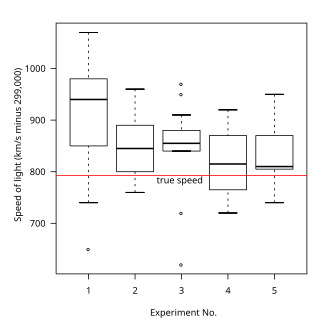
\includegraphics[height=6cm]{Pictures/data/data_box-plot.jpg}
    \caption{Graph: Box Plot}
\end{figure}
